
\section{Introduction}\label{sec:chap1_intro}
 
Lionel Messi's ascension from a gifted youth prospect to a global football icon 
unfolded over a remarkable period at FC Barcelona.
His time with the Catalan giants serves as a testament to both extraordinary 
talent and unwavering dedication, ultimately elevating him to a status few 
athletes ever achieve. 

This chapter examines the formative years of Messi's legendary career.
By analyzing his performances, his unparalleled success in winning titles, and 
the transformative impact he had on FC Barcelona, the groundwork for 
understanding his enduring influence on the sport is established.
His successes are reflected in titles, such as \textcite{messi2011ucl} 
and \textcite{messi2015ucl}, and in astounding individual performances
\parencite[e.g,][]{messi2009clasico}.

This exploration sets the stage for the dissertation's subsequent analysis of 
Messi's continued evolution throughout his career, 
including the challenges and triumphs he faced beyond Barcelona's hallowed grounds. 

This chapter is organized as follows. 
Section \ref{sec:chap1_background} provides background information on Messi's 
early years at FC Barcelona.
Section \ref{sec:chap1_titles} presents an overview of the titles Messi won 
during his time at the club.
Section \ref{sec:chap1_performance} analyzes Messi's performance metrics during 
his tenure at FC Barcelona.

\section{Background}\label{sec:chap1_background}

Lionel Messi joined FC Barcelona's youth academy, La Masia, at the age of 13.
His prodigious talent was evident from an early age, and he quickly rose through
the ranks of the club's youth system.

Messi made his first-team debut for Barcelona in 2004, at the age of 17.
He quickly established himself as a key player for the club, showcasing his
remarkable dribbling ability, vision, and goal-scoring prowess.

\section{Titles}\label{sec:chap1_titles}

During his time at FC Barcelona, Lionel Messi won numerous titles, as depicted
in Table \ref{tab:messi_barca_titles}.
These include multiple La Liga titles, UEFA Champions League titles, and Copa del Rey
titles.

\begin{table}[ht!]
    \centering
    \caption{Lionel Messi's Titles with FC Barcelona}
    \begin{tabular}{|c|c|}
    \hline
    \textbf{Competition} & \textbf{Number of Titles} \\ \hline
    La Liga & 10 \\ \hline
    Copa del Rey & 7 \\ \hline
    UEFA Champions League & 4  \\ \hline
    \end{tabular}
    \label{tab:messi_barca_titles} 
\end{table}
    

His position in the field and playing style evolved over the years, as 
different coaches utilized his talents in various ways.
For example, under Pep Guardiola, Messi played as a false nine, dropping deep
to create space for his teammates and exploit opposition defenses.
This constant evolution and adaptation to different roles on the field
demonstrate Messi's versatility and footballing intelligence, and were 
key to his success at Barcelona.

\section{Performance}\label{sec:chap1_performance}

Messi had a record-breaking season in 2012, scoring 91 goals in all competitions.
This peak performance is illustrated in Figure \ref{fig:messi_goals_xg_2012}, which
shows the ratio of goals to expected goals (xG) for Messi and other players.
Messi consistently outperformed his xG, demonstrating his exceptional finishing
ability and efficiency in front of goal.

\begin{figure}[ht!]
    \centering
    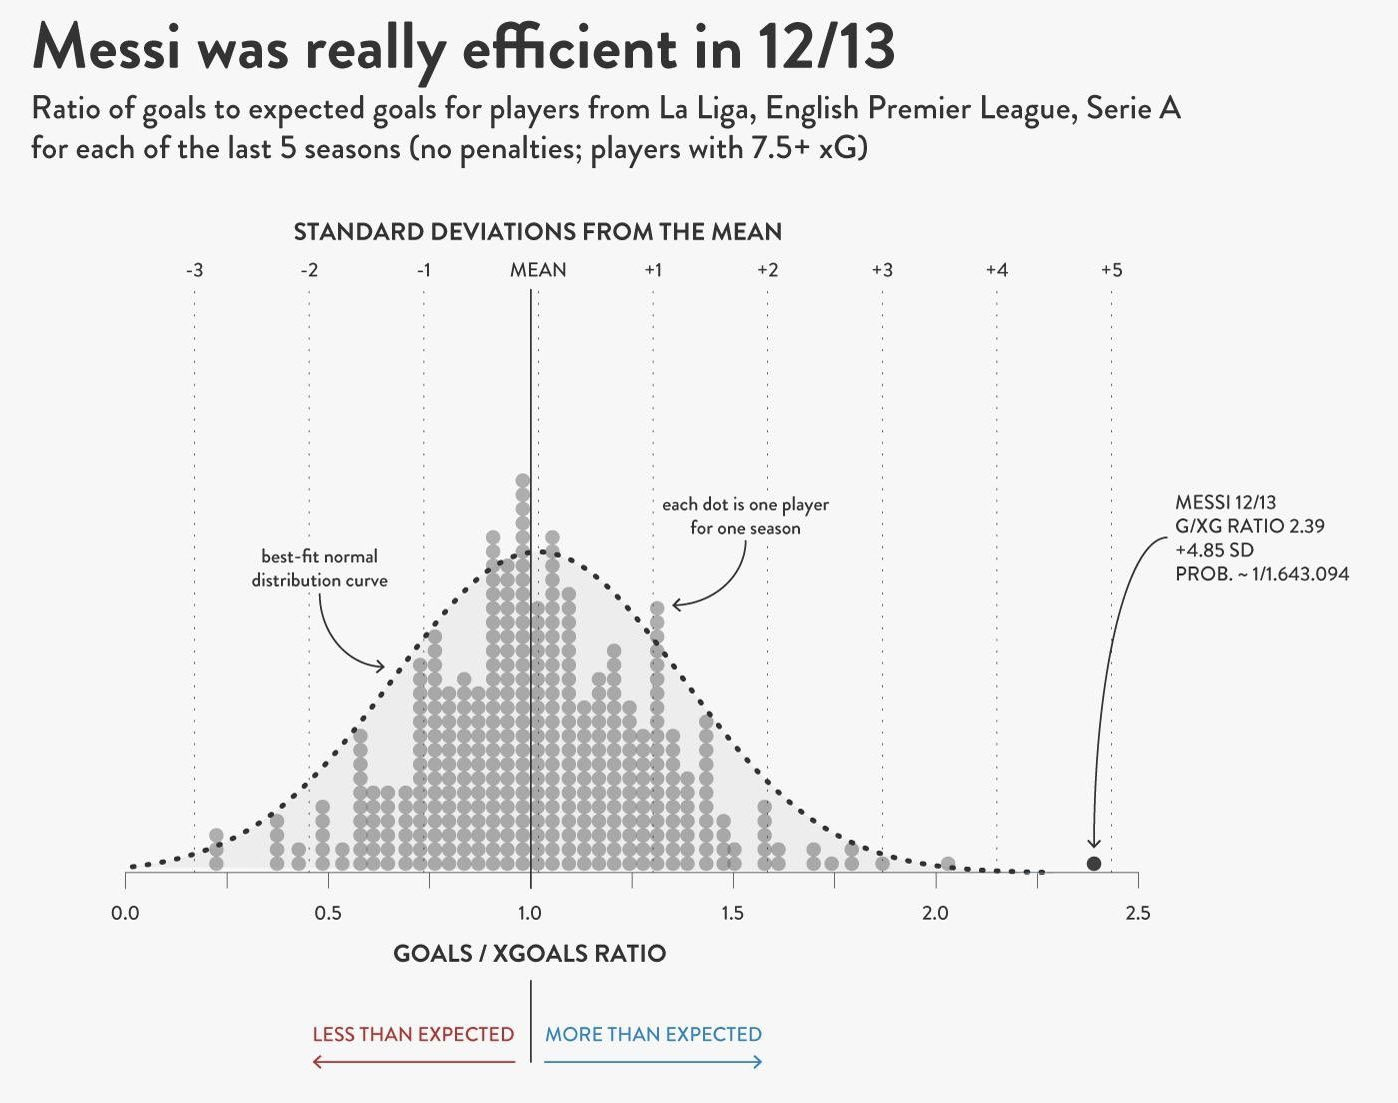
\includegraphics[width=0.7\textwidth]{graphics/messi_2012.jpg}
    \caption{Messi's Exceptional Finishing in 2012/13}
    \label{fig:messi_goals_xg_2012}
    \begin{quote}
        \textit{Notes:} 
        The figure shows the ratio of goals to expected goals (xG) for several 
        players in the 2012/13 season.
        \textit{Source:} Twitter, @xGPhilosophy.
    \end{quote} 
\end{figure}


Messi's performances resulted in multiple awards and accolades.
For instance, Appendix \ref{sec:ballon_dor} provides a summary of Messi's Ballon 
d'Or awards, highlighting his dominance in world football during his time 
at Barcelona.


